\section{Method}
\subsection{Problem Setup and Overview}
We consider a single, fixed multimodal teacher with three branches: a text branch \(f^{(t)}\), a vision branch \(f^{(v)}\), and a lightweight fusion branch \(f^{(f)}\). For notational convenience we refer to these branches as ``teachers'' or ``views.'' The student \(s_\theta\) shares the same encoders with a fusion head of comparable capacity, but only the student parameters are updated during distillation. For a post \(x=(x_{t}, x_{v})\) with label \(y\in\{0,1\}\), the task is binary misinformation detection. Let \(p^{(k)}(y\mid x)\) be the posterior of branch \(k\in\{t,v,f\}\) and \(p_\theta(y\mid x)\) that of the student. We denote the predicted class and confidence of each teacher branch by \((\hat y_k, c_k)\), where \(c_k\) is a temperature–scaled softmax score used only for gating and reliability.

Two coupled phenomena motivate \emph{selective} knowledge transfer. First, \emph{cross–modal inconsistency}: text and image may conflict (e.g., satire text plus unrelated stock photo), so copying whichever teacher is more confident can amplify errors. Second, \emph{event burstiness}: posts clustered in an event/topic \(e\) may share correlated noise. Our design therefore has two filters with distinct granularity:
an \textbf{instance–level gate} that requires cross–view agreement, and an \textbf{event–level reliability} that down–weights unreliable topics. Throughout, the selected modality \(m\in\{t,v\}\) is chosen per instance by a lightweight selector (default: the teacher with higher calibrated confidence), while the fusion teacher provides a consensus view.

% Framework figure (two-column)
\begin{figure*}[t]
  \centering
  \IfFileExists{figures/figure.png}{%
    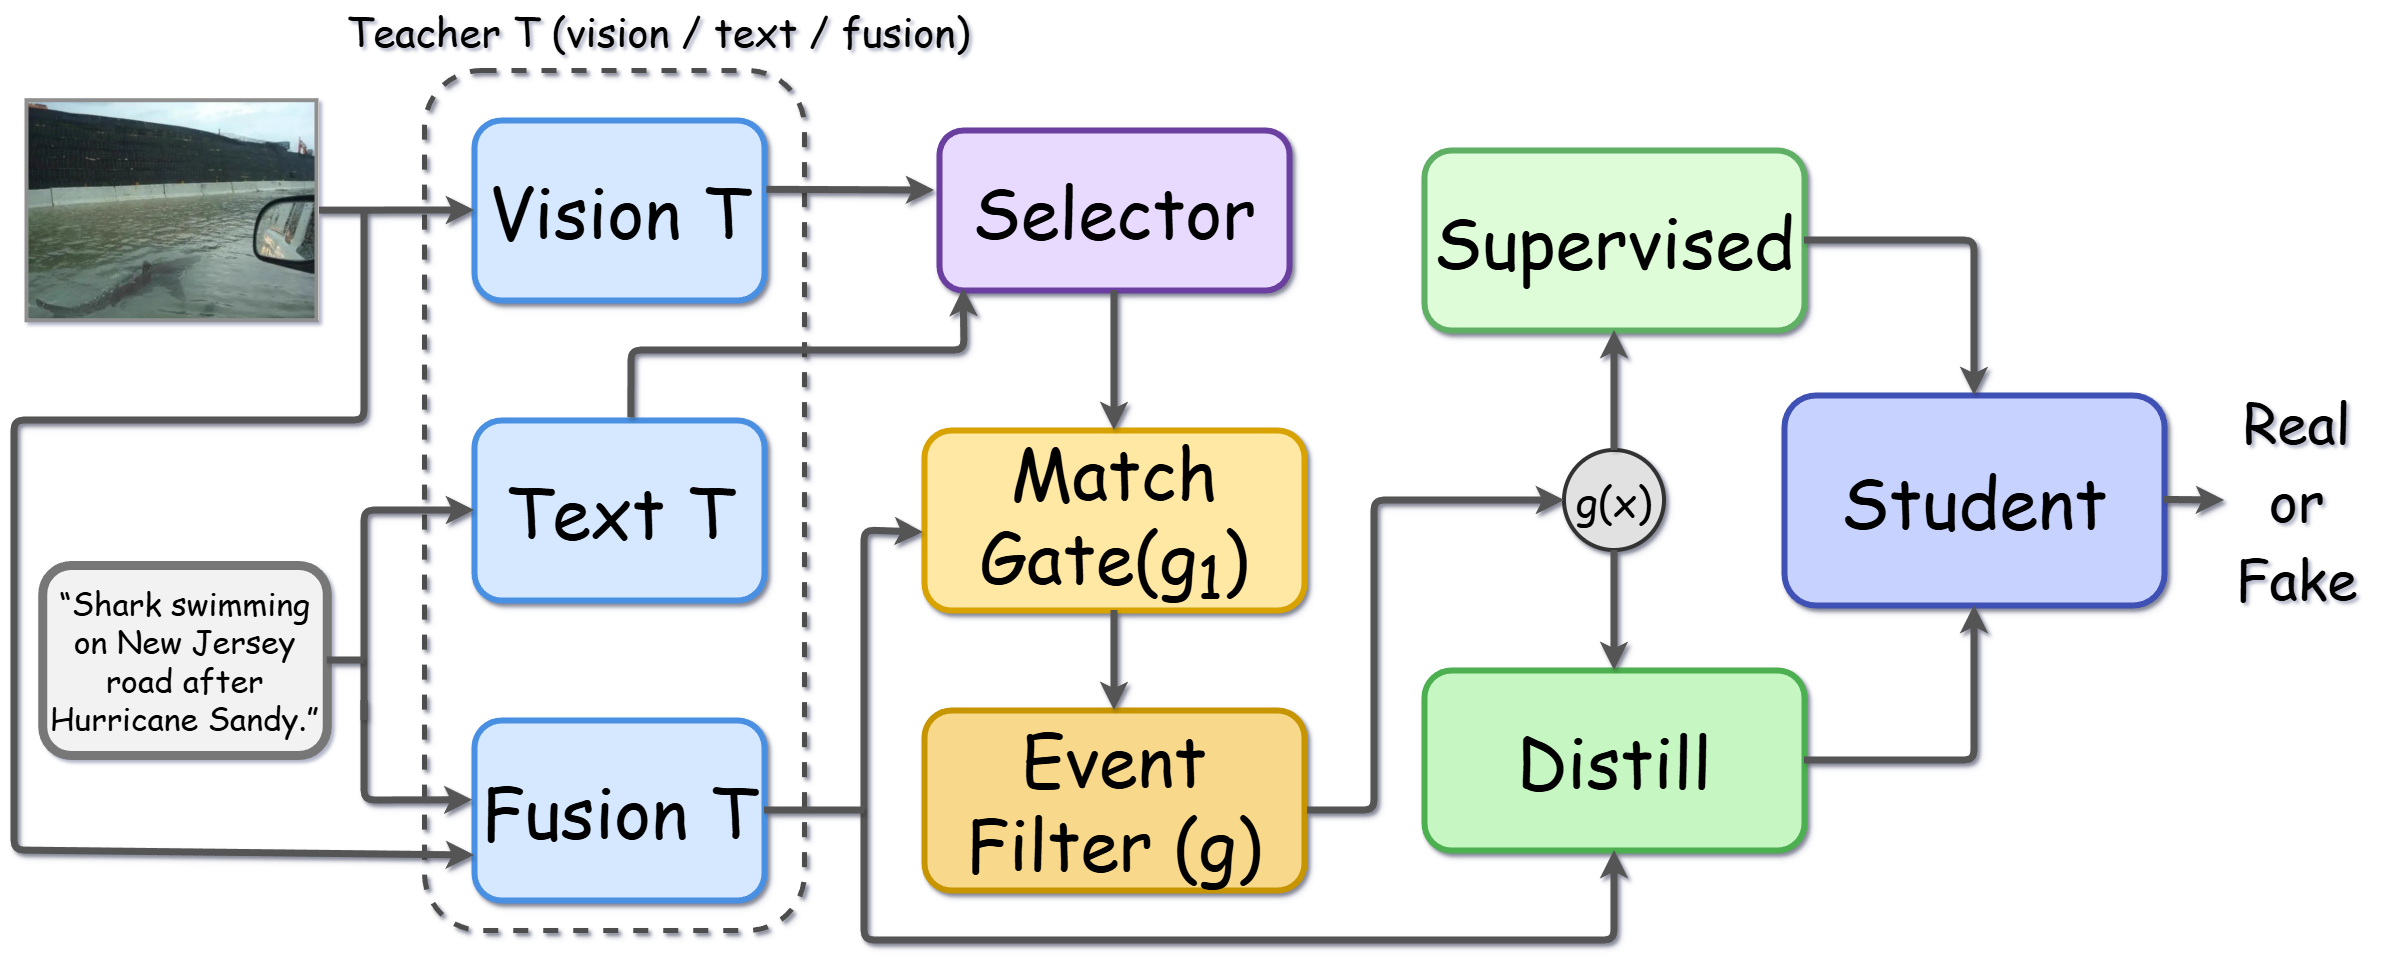
\includegraphics[width=0.98\textwidth]{figures/figure.png}%
  }{%
    \fbox{\rule{0pt}{140pt}\rule{0.98\textwidth}{0pt}}%
  }
  \caption{Overview of \modelname{}. The dashed box denotes the multimodal teacher with vision, text, and fusion branches. A selector picks the more reliable unimodal branch, and the match gate checks its agreement with the fusion branch. The event filter incorporates event-level reliability to produce the final gate $g(x)$, which controls whether the student receives distillation from the fusion teacher or is trained only with supervised losses. At test time, only the student is used to predict real or fake.}
  \label{fig:framework}
\end{figure*}

\subsection{Teacher–Match Gating}
For brevity, denote the fused teacher by $(\hat{y}_f,c_f)$
and the selected-modality teacher by $(\hat{y}_m,c_m)$.
The gate maps an instance to $\{0,1\}$:
\begin{equation}
g(x)=
\begin{cases}
1, &
\begin{aligned}[t]
&\text{if } \hat{y}_f=\hat{y}_m,\; c_f\ge\tau_f,\\
& c_m\ge\tau_m,\; \lvert c_f-c_m\rvert\le\delta,
\end{aligned}
\\[2pt]
0, & \text{otherwise.}
\end{cases}
\end{equation}

Here $\delta$ is a confidence-gap margin and temperatures $T$ modulate softmax sharpness. Intuitively, the gate admits a sample only when (i) fusion and the selected modality predict the \emph{same} class and (ii) both are confident without disagreeing in magnitude. This conservative rule privileges cross–view consensus and avoids copying high–confidence mistakes \citep{BlumMitchell1998}. When the gate is open (\(g(x)=1\)), the distillation target is taken from the teachers; otherwise the student falls back to supervised terms only (cf. the objective below).

\subsection{Event–Level Reliability}
Each post is assigned to an event/topic \(e\) (rumor or news story IDs, conversation roots on threaded platforms, or public-account stories in WeChat/WeFEND). In our experiments we use the explicit event IDs provided by Weibo and WeFEND; for datasets without such IDs (e.g., MiRAGeNews) we do not apply event-level filtering and only use instance-level gating. We track a reliability score \(r_e\in[0,1]\) by an exponential moving average (EMA) over past teacher outcomes within that event: \(r_e\leftarrow (1-\beta)\, r_e + \beta\, \mathbb{1}[\text{teacher correct}]\), where correctness is measured against ground-truth labels on the training set only. We also maintain a companion EMA of mean confidence. During training, if the event reliability drops below a cutoff or confidence is persistently low, we force the gate to close for that event (i.e., treat it as \(g(x)=0\) irrespective of instance cues). This decouples learning from bursts of correlated noise and echoes curriculum/mentor ideas under noise \citep{MentorNet2018,Han2018Coteaching}. At test time, $r_e$ is not updated.

\subsection{Calibration–Oriented Objective}
Let $q$ be the teacher target used when the gate admits a sample (fusion or the selected modality), and let $h_\theta, h^{(f)}$ be the student and fusion features. We anneal temperatures and margins over the training fraction $\lambda\in[0,1]$. The objective below decomposes into short, named terms to make the roles of distillation, supervision, feature alignment and calibration explicit:

\begingroup\small
\begin{equation}\label{eq:obj}
\begin{split}
\mathcal{L}
  &= \lambda_{\mathrm{ce}} L_{\mathrm{ce}}
   + \lambda_{\mathrm{kl}} L_{\mathrm{kl}}
   + \lambda_{\mathrm{feat}} L_{\mathrm{feat}}
   + \lambda_{+} L_{+}
   + \lambda_{\mathrm{evi}} L_{\mathrm{evi}},\\[-2pt]
&\text{where } 
\begin{aligned}[t]
L_{\mathrm{kl}}   &= \mathrm{KL}\!\left(q_T \,\Vert\, p_{\theta,T}\right),\\
L_{\mathrm{feat}} &= \lVert h_{\theta}-h^{(f)}\rVert_2^{2},\\
L_{+}             &= \mathbf{1}\{y=1\}\,\mathrm{CE}(p_{\theta},y),\\
L_{\mathrm{ce}}   &= \mathrm{CE}(p_{\theta},y)
\end{aligned}
\end{split}
\end{equation}
\endgroup
where temperature $T$ controls sharpness, the positive–class term combats imbalance, and $\mathcal{L}_{\mathrm{evi}}$ discourages unwarranted certainty \citep{Sensoy2018EDL}. When the gate is closed, the loss reduces to the supervised components ($L_{\mathrm{ce}}$ and $L_{+}$); when open, the KL and feature alignment terms engage. For reporting calibration, we apply post–hoc temperature scaling on validation as in \citet{Guo2017Calibration}.

\paragraph{Evidential Head.} We parameterize a Dirichlet distribution over class probabilities with concentration $\boldsymbol{\alpha}=\boldsymbol{e}+\mathbf{1}$, where nonnegative evidence $\boldsymbol{e}$ is predicted by a small head. The total evidence $S=\sum_c \alpha_c$ controls confidence. We use a standard evidential loss that combines a supervised term (encouraging large evidence for the true class) with a regularizer that penalizes excessive evidence on misfit examples, promoting calibrated uncertainty \citep{Sensoy2018EDL}.

\subsection{Optimization and Scheduling}
We use a simple schedule that mirrors the roles of the gate and reliability:
\emph{warm–up} (no KD; stabilize supervised prediction), then \emph{distillation} with progressively tighter thresholds and cooler temperatures, and finally an optional \emph{fine–tune} (no KD) for calibration. Concretely, thresholds \(\tau_f(\lambda),\tau_m(\lambda)\) increase and the margin \(\delta(\lambda)\) decreases with \(\lambda\); the event cutoff \(\rho(\lambda)\) increases to be more conservative late in training. Hyper–parameters and defaults are specified in the anonymized supplementary material; encoders follow \citet{Devlin2019BERT,Dosovitskiy2020ViT}.

\subsection{Algorithm and Complexity}
At each step, we compute teacher posteriors, evaluate the gate and event reliability, form \(q\) if selected, and update \(\theta\) by backpropagating \(\mathcal{L}\). The additional cost is a few softmaxes and vector operations per instance; in our implementation, teachers run in inference mode and their features can be cached when memory permits. The per–batch overhead is negligible relative to encoder forward passes. We ablate caching and scheduling choices in Section~\ref{sec:experiments}.

\begin{center}
\begin{minipage}{0.97\linewidth}
\begin{small}
\textbf{Algorithm 1: DMPD with teacher–match gate and event reliability}\\
\textit{Inputs:} teachers $f^{(t)}, f^{(v)}, f^{(f)}$; student $s_\theta$; selector for modality $m\in\{t,v\}$ (default: higher \emph{calibrated} confidence); thresholds $(\tau_f,\tau_m,\delta,\rho)$; schedules for $T$ and weights.\\
\textit{State:} event reliability $r_e$ (EMA), confidence EMA per event.
\begin{enumerate}
  \item For each minibatch $(x,y,e)$ and training fraction $\lambda$: compute $p^{(k)}(\cdot\mid x)$ for $k\in\{t,v,f\}$ and student $p_\theta$; choose $m\in\{t,v\}$ by calibrated confidence.
  \item Gate: if $\hat y^{(f)}=\hat y^{(m)}$, $c^{(f)}\!\ge\!\tau_f(\lambda)$, $c^{(m)}\!\ge\!\tau_m(\lambda)$ and $|c^{(f)}-c^{(m)}|\le\delta(\lambda)$, set $g(x)=1$; else 0.
  \item Event filter: if $r_e\!<\!\rho(\lambda)$ or mean confidence low, force $g(x)=0$.
  \item If $g(x)=1$, set distillation target $q$ (fusion or modality) and compute $\mathcal L$; otherwise train with supervised terms only.
  \item Update $\theta$ and event statistics (EMA of correctness/confidence).
\end{enumerate}
\end{small}
\end{minipage}
\end{center}

\subsection{Connections and Failure Modes}
DMPD relates to co–training by leveraging cross–view agreement \citep{BlumMitchell1998}, but the agreement is enforced between branches of a single multimodal teacher rather than two independently trained models. It also connects to curriculum/mentor methods under label noise \citep{MentorNet2018,Han2018Coteaching}: event-level reliability plays the role of a topic-level curriculum that down-weights historically unreliable events. Compared to simple confidence-based pseudo-labeling or Noisy Student-style self-training \citep{Xie2020NoisyStudent}, DMPD uses soft teacher distributions, explicit cross-view checks, and event-aware gating instead of per-instance confidence thresholds alone. Finally, it is linked to uncertainty–aware calibration \citep{Guo2017Calibration,Sensoy2018EDL} through temperature-aware KL and evidential regularization. Failure modes include (i) systemic teacher bias where all branches agree but are wrong, and (ii) over–filtering that under–trains rare but important positives. Event reliability and positive–class costs mitigate these risks; targeted ablations and error analyses are provided.

\paragraph{Scope and Assumptions.} DMPD assumes access to a moderately strong multimodal teacher with explicit text, vision, and fusion branches, and supervised event IDs at training time. If the teacher is highly inaccurate or systematically biased on most events, or if event structure is unavailable, filtering based on teacher agreement and event reliability offers limited benefit and we rely on instance-level gating only. In practice we target settings where the teacher achieves competitive accuracy but still suffers from over-confidence and event-level noise (Weibo, WeFEND, MiRAGeNews). Extremely challenging regimes with very weak teachers (e.g., strict time-split Fakeddit) are treated as hard cases in our analysis rather than primary evaluation scenarios.
